\documentclass{article}
\usepackage[UTF8]{ctex}
\usepackage[T1]{fontenc}
\usepackage[utf8]{inputenc}
\usepackage{float}
\usepackage{placeins}
\usepackage{latexsym}
\usepackage{amsmath}
\usepackage{amsthm}
\usepackage{amssymb}
\usepackage{listings}
\usepackage{xcolor}
\usepackage{ulem}
\usepackage{multicol}
\usepackage{geometry}
\usepackage{hyperref}
\usepackage{tikz}
\usetikzlibrary{positioning}
\usetikzlibrary[arrows, shapes, chains]
\hypersetup{
	colorlinks=true,
	urlcolor=black,
}
\lstset
{
    basicstyle = \ttfamily,
    keywordstyle = \bfseries\color{blue!70},
    commentstyle = \songti \upshape,
    escapeinside=``,
    breaklines = true,
    breakatwhitespace = true,
    breakautoindent = true,
    texcl = true,
    showstringspaces = false,
    basewidth = 0.5em,
    flexiblecolumns,
    columns = fixed,
    frame = {},
}
\lstdefinestyle{C}
{
    language = C,
}
\lstdefinestyle{Assembler}
{
    language = [X86masm]Assembler,
    alsolanguage = C,
}

\title{Homework 11}
\author{PB17000297 罗晏宸}
\date{November 18 2019}


\begin{document}

\maketitle

\section*{Exercise 1}
针对\href{http://staff.ustc.edu.cn/~qlzheng/compiler/lec10_2.ppt}{第十二讲 代码优化(2)}P55上流图,计算活跃变量数据流方程。

\begin{figure}[H]
    \centering
    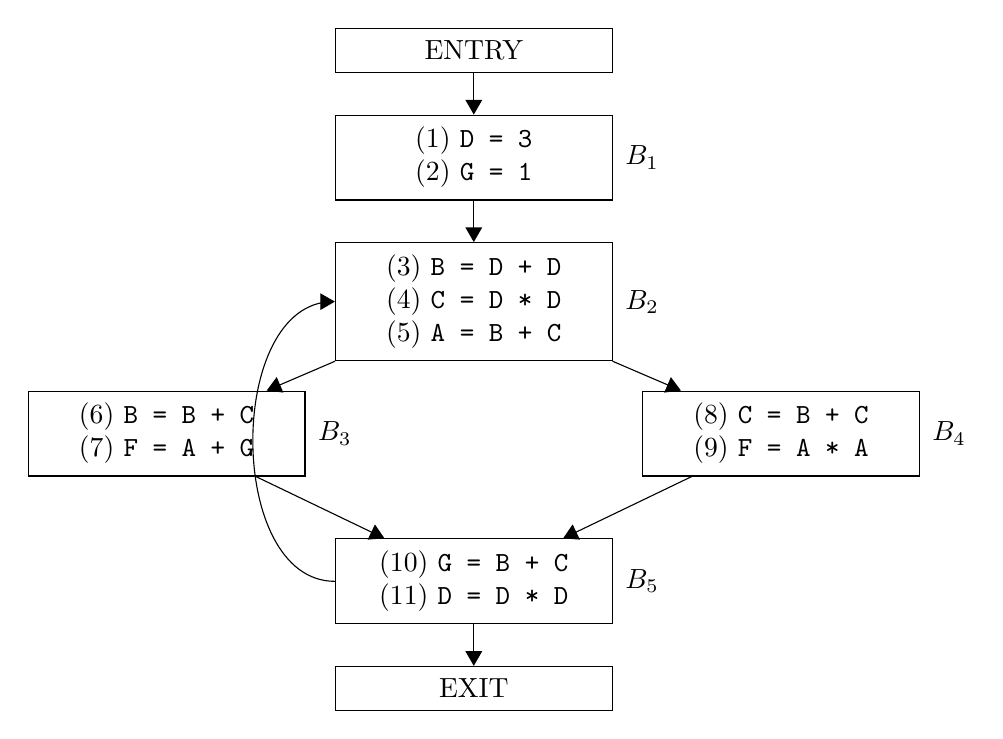
\begin{tikzpicture}[node distance = 1.5em]
        \tikzstyle{block} = [rectangle, draw=black, text ragged, minimum height = 1.6em, minimum width = 10em];
        \node [block]   (B0) {ENTRY};
        \node [block, below = of B0]   (B1)
        {
            \begin{tabular}{l}
                (1) \texttt{D = 3} \\
                (2) \texttt{G = 1}
            \end{tabular}
        };
        \node [block, below = of B1]  (B2)
        {
            \begin{tabular}{l}
                (3) \texttt{B = D + D} \\
                (4) \texttt{C = D * D} \\
                (5) \texttt{A = B + C}
            \end{tabular}
        };
        \node [block, below left = of B2]  (B3)
        {
            \begin{tabular}{l}
                (6) \texttt{B = B + C} \\
                (7) \texttt{F = A + G}
            \end{tabular}
        };
        \node [block, below right = of B2]  (B4)
        {
            \begin{tabular}{l}
                (8) \texttt{C = B + C} \\
                (9) \texttt{F = A * A}
            \end{tabular}
        };
        \node [block, below = 6.4em of B2]  (B5)
        {
            \begin{tabular}{l}
                (10) \texttt{G = B + C} \\
                (11) \texttt{D = D * D}
            \end{tabular}
        };
        \node [block, below = of B5]  (B6) {EXIT};

        \foreach \i in {1, ..., 5}
            \node [right = 0.1em of B\i] (A\i) {$B_{\i}$};

        \foreach \i/\j in {0/1, 1/2, 2/3, 2/4, 3/5, 4/5, 5/6}
            \draw [-triangle 60] (B\i) to [] (B\j);

        \draw [-triangle 60] (B5) to [out = 180, in = 180] (B2);

    \end{tikzpicture}
    \caption{第十二讲 代码优化(2)P55上流图}
\end{figure}

\paragraph{解}
首先给出每个基本块的$\textit{use}$和$\textit{def}$集合
\begin{table}[H]
    \centering
    \begin{tabular}{|c|c|c|}
    \hline
    基本块 & $\textit{use}$ & $\textit{def}$ \\ \hline
    $B_1$ & $\textit{use}_1 = \{\}$ & $\textit{def}_1 = \{\texttt{D},\texttt{G}\}$ \\ \hline
    $B_2$ & $\textit{use}_2 = \{\texttt{D}\}$ & $\textit{def}_2 = \{\texttt{B},\texttt{C}\}$ \\ \hline
    $B_3$ & $\textit{use}_3 = \{\texttt{A},\texttt{B},\texttt{C},\texttt{G}\}$ & $\textit{def}_3 = \{\texttt{F}\}$ \\ \hline
    $B_4$ & $\textit{use}_4 = \{\texttt{A},\texttt{B},\texttt{C}\}$ & $\textit{def}_4 = \{\texttt{F}\}$ \\ \hline
    $B_5$ & $\textit{use}_5 = \{\texttt{B},\texttt{C},\texttt{D}\}$ & $\textit{def}_5 = \{\texttt{G}\}$ \\ \hline
    \end{tabular}
\end{table}
初始值
\begin{align*}
   & \text{IN}[B_1] = \text{IN}[B_2] = \text{IN}[B_3] = \text{IN}[B_4] = \text{IN}[B_5] = \varnothing \\
   & \text{OUT}[B_5] = \varnothing
\end{align*}
第一次迭代
\begin{align*}
    & \text{OUT}[B_5] &&= \text{OUT}[B_5] \cup \text{IN}[B_2]    &&= \{  \} \cup \{  \} &&= \{  \} \\
    & \text{IN}[B_5]  &&= \textit{use}_5 \cup ( \text{OUT}[B_5] - \textit{def}_5 ) &&= \{\texttt{B},\texttt{C},\texttt{D}\} \cup ( \{  \} - \{\texttt{G}\} ) &&= \{\texttt{B},\texttt{C},\texttt{D}\} \\
    & \text{OUT}[B_4] &&= \text{OUT}[B_4] \cup \text{IN}[B_5]    &&= \{  \} \cup \{\texttt{B},\texttt{C},\texttt{D}\} &&= \{\texttt{B},\texttt{C},\texttt{D}\} \\
    & \text{IN}[B_4]  &&= \textit{use}_4 \cup ( \text{OUT}[B_4] - \textit{def}_4 ) &&= \{\texttt{A},\texttt{B},\texttt{C}\} \cup ( \{\texttt{B},\texttt{C},\texttt{D}\} - \{\texttt{F}\} ) &&= \{\texttt{A},\texttt{B},\texttt{C},\texttt{D}\} \\
    & \text{OUT}[B_3] &&= \text{OUT}[B_3] \cup \text{IN}[B_5]    &&= \{  \} \cup \{\texttt{B},\texttt{C},\texttt{D}\} &&= \{\texttt{B},\texttt{C},\texttt{D}\} \\
    & \text{IN}[B_3]  &&= \textit{use}_3 \cup ( \text{OUT}[B_3] - \textit{def}_3 ) &&= \{\texttt{A},\texttt{B},\texttt{C},\texttt{G}\} \cup ( \{\texttt{B},\texttt{C},\texttt{D}\} - \{\texttt{F}\} ) &&= \{\texttt{A},\texttt{B},\texttt{C},\texttt{D},\texttt{G}\} \\
    & \text{OUT}[B_2] &&= \text{OUT}[B_2] \cup \text{IN}[B_3] \cup \text{IN}[B_4]    &&= \{  \} \cup \{\texttt{A},\texttt{B},\texttt{C},\texttt{D},\texttt{G}\} \cup \{\texttt{A},\texttt{B},\texttt{C},\texttt{D}\} &&= \{\texttt{A},\texttt{B},\texttt{C},\texttt{D},\texttt{G}\} \\
    & \text{IN}[B_2]  &&= \textit{use}_2 \cup ( \text{OUT}[B_2] - \textit{def}_2 ) &&= \{\texttt{D}\} \cup ( \{\texttt{A},\texttt{B},\texttt{C},\texttt{D},\texttt{G}\} - \{\texttt{B},\texttt{C}\} ) &&= \{\texttt{A},\texttt{D},\texttt{G}\} \\
    & \text{OUT}[B_1] &&= \text{OUT}[B_1] \cup \text{IN}[B_2]    &&= \{  \} \cup \{\texttt{A},\texttt{D},\texttt{G}\} &&= \{\texttt{A},\texttt{D},\texttt{G}\} \\
    & \text{IN}[B_1]  &&= \textit{use}_1 \cup ( \text{OUT}[B_1] - \textit{def}_1 ) &&= \{  \} \cup ( \{\texttt{A},\texttt{D},\texttt{G}\} - \{\texttt{D},\texttt{G}\} ) &&= \{ \texttt{A} \}
\end{align*}
第二次迭代
\begin{align*}
    & \text{OUT}[B_5] &&= \text{OUT}[B_5] \cup \text{IN}[B_2]    &&= \{  \} \cup \{\texttt{A},\texttt{D},\texttt{G}\} &&= \{\texttt{A},\texttt{D},\texttt{G}\} \\
    & \text{IN}[B_5]  &&= \textit{use}_5 \cup ( \text{OUT}[B_5] - \textit{def}_5 ) &&= \{\texttt{B},\texttt{C},\texttt{D}\} \cup ( \{\texttt{A},\texttt{D},\texttt{G}\} - \{\texttt{G}\} ) &&= \{\texttt{A},\texttt{B},\texttt{C},\texttt{D}\} \\
    & \text{OUT}[B_4] &&= \text{OUT}[B_4] \cup \text{IN}[B_5]    &&= \{\texttt{B},\texttt{C},\texttt{D}\} \cup \{\texttt{A},\texttt{B},\texttt{C},\texttt{D}\} &&= \{\texttt{A},\texttt{B},\texttt{C},\texttt{D}\} \\
    & \text{IN}[B_4]  &&= \textit{use}_4 \cup ( \text{OUT}[B_4] - \textit{def}_4 ) &&= \{\texttt{A},\texttt{B},\texttt{C}\} \cup ( \{\texttt{A},\texttt{B},\texttt{C},\texttt{D}\} - \{\texttt{F}\} ) &&= \{\texttt{A},\texttt{B},\texttt{C},\texttt{D}\} \\
    & \text{OUT}[B_3] &&= \text{OUT}[B_3] \cup \text{IN}[B_5]    &&= \{\texttt{B},\texttt{C},\texttt{D}\} \cup \{\texttt{A},\texttt{B},\texttt{C},\texttt{D}\} &&= \{\texttt{A},\texttt{B},\texttt{C},\texttt{D}\} \\
    & \text{IN}[B_3]  &&= \textit{use}_3 \cup ( \text{OUT}[B_3] - \textit{def}_3 ) &&= \{\texttt{A},\texttt{B},\texttt{C},\texttt{G}\} \cup ( \{\texttt{A},\texttt{B},\texttt{C},\texttt{D}\} - \{\texttt{F}\} ) &&= \{\texttt{A},\texttt{B},\texttt{C},\texttt{D},\texttt{G}\} \\
    & \text{OUT}[B_2] &&= \text{OUT}[B_2] \cup \text{IN}[B_3] \cup \text{IN}[B_4]    &&= \{\texttt{A},\texttt{B},\texttt{C},\texttt{D},\texttt{G}\} \cup \{\texttt{A},\texttt{B},\texttt{C},\texttt{D},\texttt{G}\} \cup \{\texttt{A},\texttt{B},\texttt{C},\texttt{D}\} &&= \{\texttt{A},\texttt{B},\texttt{C},\texttt{D},\texttt{G}\} \\
    & \text{IN}[B_2]  &&= \textit{use}_2 \cup ( \text{OUT}[B_2] - \textit{def}_2 ) &&= \{\texttt{D}\} \cup ( \{\texttt{A},\texttt{B},\texttt{C},\texttt{D},\texttt{G}\} - \{\texttt{B},\texttt{C}\} ) &&= \{\texttt{A},\texttt{D},\texttt{G}\} \\
    & \text{OUT}[B_1] &&= \text{OUT}[B_1] \cup \text{IN}[B_2]    &&= \{\texttt{A},\texttt{D},\texttt{G}\} \cup \{\texttt{A},\texttt{D},\texttt{G}\} &&= \{\texttt{A},\texttt{D},\texttt{G}\} \\
    & \text{IN}[B_1]  &&= \textit{use}_1 \cup ( \text{OUT}[B_1] - \textit{def}_1 ) &&= \{  \} \cup ( \{\texttt{A},\texttt{D},\texttt{G}\} - \{\texttt{D},\texttt{G}\} ) &&= \{ \texttt{A} \}
\end{align*}
计算结果不再改变,迭代终止。
\end{document}

